% !TEX encoding   = UTF8
% !TEX spellcheck = ru_RU
% !TEX root = ../seminars.tex

%%====================================
\chapter{Ассемблирование и компоновка}
%%====================================
В~качестве примера рассмотрим следующую программу, состоящую из~двух модулей:

\medskip\noindent
\begin{minipage}[t]{0.5\textwidth}
  \begin{flushleft}
    \underline{\code{main.c}}
  \end{flushleft}
  \cfile{projects/sem13/main.c}
\end{minipage}%
%
\begin{minipage}[t]{0.5\textwidth}
  \begin{flushleft}
    \underline{\code{swap.c}}
  \end{flushleft}
  \cfile{projects/sem13/swap.c}
\end{minipage}



%%=====================
\section{Стадии сборки}
%%=====================
Ключ~\code{-v} заставляет \GCC{} выводить подробную информацию о~совершаемых действиях:
\begin{consolecode}
$ gcc -Og -g -o p -v main.c swap.c
...
cc1 main.c [other arguments] -g -Og -o /tmp/ccU1HP45.s
as --64 -o /tmp/cc7TbUce.o /tmp/ccU1HP45.s
...
collect2 -m elf_x86_64 -o p [system object files and args] /tmp/cc7TbUce.o
/tmp/cc6OWLom.o -lc [other libraries]
\end{consolecode}



%%====================
\paragraph{Замечание.}
%%====================
В~современном \GCC{} препроцессор встроен в~сам компилятор \code{cc1}, поэтому нет необходимости вызывать его в~явном виде. Результат работы препроцессора (\code{main.i} и \code{swap.i}) можно получить отдельно, используя опцию \code{-save-temps}.

Утилита \code{collect2} на~самом деле является <<обёрткой>> компоновщика \code{ld} и вызывает его, выполнив перед этим (в~некоторых случаях) дополнительные действия, например, генерацию кода для~конструкторов.



%%==================================
\section{Структура объектного файла}
%%==================================
\noindent \code{ELF} = \textenglish{Executable and Linkable Format}

{\newcommand*{\segm}[1]{\hbox to 2.5cm {\code{#1}}}%
\small\begin{longtable}[l]{|c|l}
  \cline{1-1}
\endfoot
  \cline{1-1}
  \code{ELF} header & тип файла; архитектура; смещение, размер и число записей табл. заголовков \\
  \cline{1-1}
  \segm{.text}     & сегмент кода \\
  \cline{1-1}
  \segm{.rodata}   & сегмент данных с~доступом только на~чтение \\
  \cline{1-1}
  \segm{.data}     & сегмент данных с~доступом на~чтение\slash запись \\
  \cline{1-1}
  \segm{.bss}      & неинициализированные глобальные переменные \\
  \cline{1-1}
  \segm{.symtab}   & таблица символов \\
  \cline{1-1}
  \segm{.rel.text} & адреса в~коде, которые необходимо скорректировать при~компоновке \\
  \cline{1-1}
  \segm{.rel.data} & данные для~корректировки глобальных переменных, хранящих адреса \\
  \cline{1-1}
  \segm{.debug}    & таблица символов для~отладки (с~ключом~\code{-g}) \\
  \cline{1-1}
  \segm{.line}     & таблица соответствия номеров строк исх. и машинного кодов (с~ключом~\code{-g}) \\
  \cline{1-1}
  \segm{.strtab}   & таблица строк \\
  \cline{1-1}
  section header table & смещения и размеры различных сегментов объектного файла \\
  \cline{1-1}
\end{longtable}}



%%========================
\section{Таблица символов}
%%========================
Символические имена, или \emph{символы}, либо являются метками, либо определяются явным образом (при~помощи директив). В~каждой строке таблицы символов содержится само имя (или указатель на~него), его численное значение и иногда некоторая дополнительная информация. Она может включать:
\begin{itemfeature}
  \item длину поля данных, связанного с~символическим именем;
  \item биты перераспределения памяти;
  \item сведения о~том, можно ли получить доступ к~имени извне процедуры/модуля.
\end{itemfeature}

\noindent Например, символ таблицы в~\code{ELF} определяется так:
\begin{ccode}
typedef struct {
  int name;        /* string table offset */
  int value;       /* section offset, or VM address */
  int size;        /* object size in bytes */
  char type:4,     /* data, func, section, or src file name (4 bits) */
       binding:4;  /* local or global (4 bits) */
  char reserved;   /* unused */
  char section;    /* section header index, ABS, UNDEF, or COMMON */
} Elf_Symbol;
\end{ccode}

\noindent С~точки зрения компоновщика, существуют следующие виды символов:
\begin{itemfeature}
  \item \emph{глобальные}, определяются в~модуле и доступны извне. В~языке~\lang{C} они соответствуют нестатическим функциям и глобальным переменным, объявленным без~квалификатора \code{static}.

  \item \emph{внешние} "--- глобальные символы, к~которым обращается модуль, но которые определены где-то в~другом модуле.

  \item \emph{локальные}, определение и обращение к~которым происходит только внутри модуля. Некоторые локальные символы соответствуют~\lang{C} функциям и глобальным переменным, объявленным с~квалификатором \code{static}.
\end{itemfeature}



%%=====================
\paragraph{Упражнение.}
%%=====================
Выведите таблицу символов для~объектных файлов.

\begin{consolecode}
$ gcc -Og -c main.c swap.c
$ readelf --syms main.o swap.o
\end{consolecode}

\begin{textcode}
Num:    Value          Size Type    Bind   Vis      Ndx Name
File: main.o
...
  8: 0000000000000000    24 FUNC    GLOBAL DEFAULT    1 main
...
 10: 0000000000000000     0 NOTYPE  GLOBAL DEFAULT  UND swap
 11: 0000000000000000     8 OBJECT  GLOBAL DEFAULT    3 buf
File: swap.o
...
  9: 0000000000000000    41 FUNC    GLOBAL DEFAULT    1 swap
 10: 0000000000000000     0 NOTYPE  GLOBAL DEFAULT  UND buf
 11: 0000000000000008     8 OBJECT  GLOBAL DEFAULT  COM bufp1
 12: 0000000000000000     8 OBJECT  GLOBAL DEFAULT    5 bufp0
\end{textcode}

\noindent Для~каждого символа в~таблице, следующей ниже, укажите, находится ли он в~символьной таблице модуля \code{swap.o}; тип: глобальный, локальный или внешний; модуль, где находится определение символа; и сегмент, в~котором расположен символ:

\vspace{-0.5\baselineskip}
\begin{center}
\newcommand*{\ans}[2][1.5cm]{\ansfw{#1}{\hfill#2\hfill\makebox[0pt]{\phantom{p}}}}%
\newcommand*{\anstype}[1]{\ans[\widthof{глобальный}]{#1}}%
\begin{tabular}{@{}lcccr@{}}
  \textsf{Символ} & \textsf{запись в swap.o .symtab?} & тип символа & модуль, где определён & сегмент \\
\midrule
  \code{buf}   & \ans{да}  & \anstype{внешний}    & \ans{main.o} & \ans{\code{.data}} \\
  \code{bufp0} & \ans{да}  & \anstype{глобальный} & \ans{swap.o} & \ans{\code{.data}} \\
  \code{bufp1} & \ans{да}  & \anstype{глобальный} & \ans{swap.o} & \ans{\code{.bss}} \\
  \code{swap}  & \ans{да}  & \anstype{глобальный} & \ans{swap.o} & \ans{\code{.text}} \\
  \code{tmp}   & \ans{нет} & \anstype{---}        & \ans{---}    & \ans{---} \\[2pt]
\end{tabular}
\end{center}



%%======================================
\section{Ассемблирование за~два прохода}
%%======================================
\emph{Проблема опережающей ссылки}: символическое имя используется до~своего определения (то есть выполняется обращение к~символическому имени, определение которого появится позднее).



%%========================
\paragraph{Первый проход.}
%%========================
Основная задача~--- построить \emph{таблицу символических имён}.

\begin{cppcode}
void pass_one ()
{
  constexpr int END_STATEMENT {-2};
  int location_counter {0};
  int type {0};

  initialize_tables();

  do {
    string line = read_next_line();
    int length {0};
    string opcode;

    if (line_is_not_comment (line))
    {
      string symbol = check_for_symbol (line);
      if (!symbol.empty())
        enter_new_symbol (symbol, location_counter);

      string literal = check_for_literal (line);
      if (!literal.empty())
      enter_new_literal (literal);

      opcode = extract_opcode (line);
      type = search_opcode_table (opcode);

      if (type < 0)
        type = search_pseudo_table (opcode);

      switch (type)
      {
        case 1: length = get_length_of_type1 (line); break;
        case 2: length = get_length_of_type2 (line); break;
        // ...
      }
    }

    write_temp_file (type, opcode, length, line);

    location_counter += length;

  } while (type != END_STATEMENT);

  rewind_temp_for_pass_two();
  sort_literal_table();
  remove_redundant_literals();
}
\end{cppcode}



%%========================
\paragraph{Второй проход.}
%%========================
Основная задача "--- создание объектного кода и информации, необходимой для~компоновки в~исполняемый файл. Попутно вывод протокола ассемблирования, если нужно.

\begin{cppcode}
void pass_two ()
{
  constexpr int END_STATEMENT {-2};
  constexpr int MAX_CODE {16};
  char code[MAX_CODE];
  int location_counter {0};

  do {
    int type = read_type();
    int opcode = read_opcode();
    int length = read_length();
    string line = read_line();

    if (type != 0)  // if not a comment
    {
      switch (type)
      {
        case 1: eval_type1 (opcode, length, line, code); break;
        case 2: eval_type2 (opcode, length, line, code); break;
        // ...
      }
    }

    write_output (code);
    write_listing (code, line);

    location_counter += length;

  } while (type != END_STATEMENT);

  finish_up();
}
\end{cppcode}



%%==================
\section{Компоновка}
%%==================
Основные задачи:
\begin{itemfeature}[itemsep=0.5em]
  \item \emph{Идентификация символов.} Объектные файлы определяют символы и обращаются к~символам. Цель идентификации, или разрешения, символов "--- поставить каждому обращению к~символу в~соответствие единственное определение этого символа.

  \item \emph{Перераспределение адресов.} Компиляторы и ассемблеры создают сегменты кода и данных, которые начинаются с~адреса~\code{0}. Компоновщик объединяет и перераспределяет, или перемещает, эти сегменты, определяя местоположение в~памяти каждого символа, а затем корректирует все обращения к~символам так, чтобы они ссылались в~соответствующую область памяти.
\end{itemfeature}



%%==============================
\section{Загрузка на~исполнение}
%%==============================
Чтобы запусить исполняемый файл \code{prog} на~выполнение, необходимо набрать его имя в~командной оболочке:

\console`$ ./prog`

\noindent
\begin{minipage}[t]{0.5\textwidth}
\parindent=2.5em

При~этом командная оболочка вызовет системный код, называемый загрузчиком. Он скопирует код и данные из~исполняемого файла в~память, и, затем, запустит программу, передав управление первой инструкции, или \emph{точке входа}. Этот процесс называется \emph{загрузкой} на~исполнение.

\end{minipage}\hfill\begin{minipage}[t]{0.5\textwidth}

\vspace{-5em}
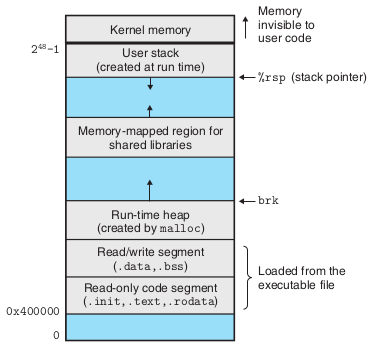
\includegraphics[width=\textwidth]{images/loaded_executable.png}

\end{minipage}



%%================
\WhatToReadSection
%%================
\begin{tabular}{@{}l@{}}
  \citeauthor[глава~7, стр.~634--660]{Bryant:2022:ru} \\
  \citeauthor[глава~7, стр.~571--592]{Tanenbaum:2007:ru}
\end{tabular}
